\chapter{Implementierung einer Progressive Web App und Native App}\label{ch:implementation}
Die Daten für die zu implementierenden Applikationen werden von der offiziellen REST\footnote{Ein gängiges Datenformat des Datenaustauschs im Web.} \ac{api} des Robert Koch-Instituts bezogen.
Sie werden täglich um Mitternacht prozessiert und sind in den frühen Morgenstunden in der \ac{api} verfügbar.
Konkret wird die Datenbank \glqq RKI Corona Landkreise\grqq{} genutzt, die die Zahlen gruppiert nach Landkreisen im Geo\ac{json} und \ac{json}-Format zur Verfügung stellt.
Sie besitzt insgesamt 2.117.948 Datensätze und als CSV-Datei eine Größe von 308 MB\cite{COVID19Datenhub.2020}.\\
Für die Darstellung der Fallzahlen wurden hierbei folgende, auf den Landkreis bezogene, Attribute ausgewählt:
\begin{itemize}
\item Art des Landkreises (\textit{BEZ})
\item Name (\textit{GEN})
\item Fälle (\textit{cases})
\item Fälle der letzten 7 Tage pro 100.000 Einwohner (\textit{cases7\_per\_100k})
\item Fallzahlen pro 100.000 Einwohner (\textit{cases\_per\_100k})
\item ID (\textit{AdmUnitId})
\item Zeitpunkt der letzten Aktualisierung der Daten (\textit{last\_update})
\end{itemize}
In der Anwendung werden die Fallzahlen zum Zweck der Übersichtlichkeit auf zwei Nachkommastellen gerundet.

Für die Implementierung der zu vergleichenden Anwendungen wurden die open-source Bibliotheken React und React Native verwendet.
React dient bei der \ac{pwa} als Unterstützung zur Entwicklung einer \ac{spa}, wohingegen React Native ein komplettes Framework zur plattformunabhängigen Entwicklung von nativen Anwendungen anbietet.
Ein Vergleich mit diesen Bibliotheken bietet sich einerseits insofern an, dass deren Grundlage dieselbe Programmierweise darstellt, nämlich das deklarative und komponentenbasierte Konzept von React.
Anderseits sind durch die Verwendung von React Native beide Technologien plattformunabhängig und bilden somit eine solide Grundlage für den Vergleich.
Diese Eigenheit der Implementierung unterscheidet sich insofern grundlegend von der tatsächlichen nativen Entwicklung, als dass diese nicht betriebssystemspezifisch stattfindet.
Dafür muss die dafür vorgesehenen Programmiersprachen und ein \ac{ide} wie Android Studio mit Kotlin und Java genutzt werden.
Trotz dieser Besonderheit wird in der vorliegenden Arbeit eine React Native App als Native App mit einer \ac{pwa} verglichen, da sich generell mit React Native alle Funktionalitäten programmieren lassen, die Native Apps anbieten.

Das Besondere bei der Entwicklung einer Native App mit React Native ist, dass dies plattformunabhängig geschieht.
Wie bereits in Kapitel \ref{ch:basics} geschildert, handelt es sich dabei um einen Prozess, der von einem JavaScript Thread über \textit{Bridges} mit einem Native Thread kommuniziert und somit zur Laufzeit native Schnittstellen und \ac{ui}-Elemente aufruft.
Dadurch kann mit JavaScript Code geschrieben werden, der zur Laufzeit sowohl Android als auch iOS Komponenten anspricht.
Um eine Funktionalität mit JavaScript implementieren zu können, muss jedoch entweder bereits eine Community Lösung einer \textit{Bridge} für diese gewollte Funktion existieren oder diese selbst entwickelt werden.\\
Beide Applikationen sind im Quelltext-Editor Visual Studio Code und bis auf Ausnahmen bei der Native App mit JavaScript programmiert.

\section{Einrichten der Entwicklungsumgebung}
\subparagraph{Progressive Web App\\}
Zum Aufsetzen der Umgebung wurde die bereits genannte Create-React-App-Toolchain verwendet.
Diese wird durch npm\footnote{ehemals Node Package Manger, Anwendung zur Installation von Node.js Packages.} mit dem Befehl \textit{npx create-react-app <Name der Anwendung>} erstellt.
Hierfür wird mindestens Node\footnote{Node.js ist eine lizenzfreie und plattformunabhängige JavaScript Entwicklungsumgebung} 10.16 und npm 5.6 benötigt.
Nachteile der Verwendung einer Toolchain sind jedoch die Abhängigkeit von den dadurch integrierten Bibliotheken und das daraus resultierende Sicherheitsrisiko. 
Auf der anderen Seite ermöglicht die Toolchain einen schnellen Einstieg zur Entwicklung einer \ac{spa}.
Dies liegt vor allem an den vorgefertigten Konfigurationen zur Vereinfachung der Programmierung wie \textit{Babel}\footnote{Compiler, der mit ECMAScript 2015 geschriebenen Code rückwärtscompatibel macht durch dafür vorgesehene Polyfills.}, \textit{ESLint}\footnote{Codeanalysetool, welches den Entwickler auf problematische Codestellen aufmerksam macht.} und \textit{Webpack}\footnote{Modulbündler, der aus vielen einzelnen Dateien, ein oder mehrere große Dateien generiert. Dies erhöht die Performance der Anwendung.}.
Create-React-App bietet außerdem eine Reihe an Templates, die das Aufsetzen einer zum Projekt passenden Entwicklungsumgebung ebenfalls erleichtern sollen.
Beispielsweise das \ac{pwa} Template, das Werkzeuge wie \textit{Workbox}\footnote{Von Google entwickelte Sammlung von JavaScript Bibliotheken zur vereinfachten Implementierung von Service Workern.} und einen vorimplementierten Service Worker mitinstalliert.
Darauf wird in dieser Anwendung verzichtet, um die Funktionsweise des Service Workers selbst programmieren zu können und diese dadurch besser zu erfassen.

Die Abbildung \ref{fig:structure_pwa} zeigt die Ordnerstruktur nach dem Aufsetzen der Anwendung per Toolchain.
 
\begin{figure}[h]
 \centering
 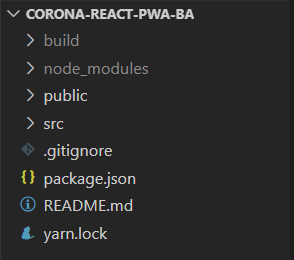
\includegraphics[width=0.6\textwidth]{figures/Structure_PWA.png}
 \caption{Ordnerstruktur Progressive Web App}
 \label{fig:structure_pwa}
\end{figure}

Im \textit{public}-Ordner befinden sich diejenigen Dateien, die an den Client versendet werden.
Konkret sind das ausgewählte Bilddateien, das App Manifest und die \textit{index.html}-Datei.
\textit{Webpack} nutzt die \textit{index.js} als Eintrittspunkt und generiert beim Ausführen der \textit{ReactDOM.render(element, document.getElementByID('root')}-Funktion einen Komponentenbaum auf dem \textit{div}-Element mit der \textit{id} \textit{root}.
Die \textit{index.js} befindet sich im \textit{src}-Ordner.
Auf ebendieser Ebene befindet sich außerdem die \textit{yarn.lock}, in der alle Abhängigkeiten der Anwendung gelistet sind, sowie die \textit{package.json}, die über Metadaten verfügt.

Mit dem Befehl \glqq npm run start\grqq{} wird eines der Skripte von Create-React-App zum Starten von \textit{Webpack} ausgeführt.
Dadurch ist die Anwendung direkt nach dem Aufsetzen unter \url{http://localhost:3000/} lokal aufrufbar.
Obwohl \text{localhost} kein \ac{https} besitzt, sind die Funktionalitäten von \acp{pwa} möglich, da es sich hierbei lediglich um die Entwicklungsumgebung handelt.

Zum Erhalten der Daten wird mit der \textit{Fetch}-Funktion eine \textit{GET}-Anfrage an die \ac{api} der Corona-Datenbank des Robert Koch-Instituts versendet und die Antwort in ein \textit{Array} gespeichert.
Dieses wird in der \textit{render}-Funktion mithilfe der \textit{Array}-Funktion \textit{map} durchlaufen.
Die Daten werden somit im \ac{ui} übersichtlich dargestellt.

Generell müssen Webanwendungen auf einen Webserver veröffentlicht werden, um im World Wide Web aufrufbar zu sein.
Speziell bei \acp{pwa} ist hierbei bedeutsam, dass dieser Webserver eine verschlüsselte Verbindung mittels \ac{https} aufbaut, da dies eine technische Voraussetzung für \acp{pwa} ist.
Zum Hosting der Webapplikation wird deshalb der Hostingservice \textit{Netlify} verwendet, welcher eine \ac{https} Verbindung bereitstellt.
Durch den Befehl \glqq npm run build\grqq{} kann eine minimierte Version der Anwendung erzeugt werden, die eine optimierte Endfassung für das Deployment der App bietet.
Nach erfolgreichem Hochladen des Build Ergebnisses ist die \ac{pwa} über den Link \url{https://corona-react-pwa-ba.netlify.app/} verfügbar.

\subparagraph{React Native App\\}
Um eine React Native Anwendung zu programmieren, gibt es zwei Ansätze: \textit{managed workflow} und \textit{bare workflow}.
Ersteres wird durch das zusätzliche Expo Framework verwaltet, das einen schnellen Einstig in die plattformunabhängige Entwicklung ermöglicht.
Diese läuft mit der zugehörigen Expo Go iOS oder Android App, indem die programmierte App in Echtzeit über einen Packager gerendert wird.
Somit kann die App sofort ohne weiteres auf dem jeweiligen Endgerät unabhängig vom Betriebssystem getestet werden.\\
Der Nachteil dieses Ansatzes ist, dass mit Expo kein nativer Code für die genannten Betriebssysteme programmiert werden kann und dadurch die Funktionalitäten auf die von Expo angebotenen \ac{api}s beschränkt sind.
Für die Funktionen, die in dieser Arbeit betrachtet werden, würde Expo ausreichen, jedoch soll an dieser Stelle kein weiteres Framework genutzt werden.
Deshalb wird der \textit{bare workflow} verwendet.\\
%Auch hier kann mit JavaScipt (oder TypeScript falls gewünscht) programmiert werden, zusätzlich besteht aber auch die Möglichkeit nativen Code zu implementieren.
Doch auch dieser Ansatz besitzt einen Nachteil.
Denn trotz der eigentlich plattformunabhängigen Entwicklungsweise besteht keine Möglichkeit, mit Windows oder Linux eine iOS App zu programmieren.
Laut der Dokumentation von React Native wird hierfür macOS benötigt.\\
Im Folgenden wird daher die Implementierung einer Android App mit React Native beschrieben und die Umsetzung derselben Funktionalitäten auf iOS nur skizziert.
Wichtig ist dabei, dass aus dem vorliegenden Code trotzdem eine iOS App erzeugt werden könnte.
Die gleiche Funktionalität wie bei der Android App ist jedoch meist nicht ohne weitere Anpassungen wie das Zulassen von Berichtigungen über Apples \ac{ide} XCode verfügbar.

Zur Erstellung eines React Native Projekts wird der Befehl \textit{npx react-native init <Name der Anwendung>} verwendet, der ebenfalls von npm zur Verfügung gestellt wird.
Außerdem müssen diejenigen Einstellungen in der Entwicklungsumgebung vorgenommen werden, die auch zur Programmierung von nativen Android Apps benötigt werden.
Das betrifft beispielsweise das Installieren von Android Studio und der Android \ac{apk}.
Nach dem Ausführen des Befehls liegt die Ordnerstruktur vor, die in der Abbildung \ref{fig:structure_rn} dargestellt ist.

\begin{figure}[h]
 \centering
 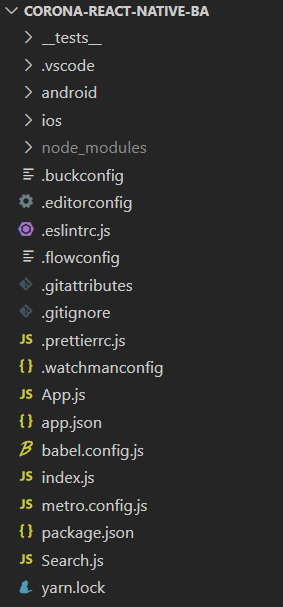
\includegraphics[width=0.4\textwidth]{figures/Structure_RN.png}
 \caption{Ordnerstruktur React Native App}
 \label{fig:structure_rn}
\end{figure}

Die Ordner \textit{ios} und \textit{android} beinhalten plattformspezifischen Code wie die \textit{Info.plist}- und die \textit{AndroidManifest.xml}-Datei, die Metainformationen über die Anwendung bereitstellen.
Auf derselben Ebene befindet sich die \textit{App.js}-Datei, in der die Anwendung mit JavaScript implementiert wird.

Um die Corona-Daten in der React Native App darzustellen, wird ebenfalls die \textit{Fetch} \ac{api} genutzt.
Diese verwendet die \textit{RCTNetworking}-Klasse als Bridge zu den nativen Modulen in Android und iOS.
In Android ist das der \textit{OkHttpClient} und in iOS \textit{XHTTP}.
Die Daten werden nach dem Abrufen durch die \textit{fetch}-Funktion in einer \textit{FlatList} angezeigt.
Der Vorteil der \textit{FlatList} ist, dass es nur diejenigen Elemente rendert, die im sichtbaren Teil des Bildschirms sind.
Dadurch werden Ressourcen gespart und das Scrollen der Liste erscheint für den Nutzer flüssiger.
Im Hintergrund spricht React Native mit der \textit{FlatList}-Komponente die Komponente \textit{ListView} in Android und in iOS an.
Die \textit{FlatList} wird umschlossen von einer \textit{SafeAreaView}-Komponente.
Dabei handelt es sich um eine iOS-spezifische Komponente, die empfohlen wird, um die \ac{ui} in iOS zu verbessern.
In der Abbildung \ref{fig:flatlist:ios} wird deutlich, welche Auswirkung das Fehlen dieser Komponente für die Benutzeroberfläche hat.

\begin{figure}
\subfigure[Darstellung einer \textit{FlatList} mit \textit{SafeViewArea}]{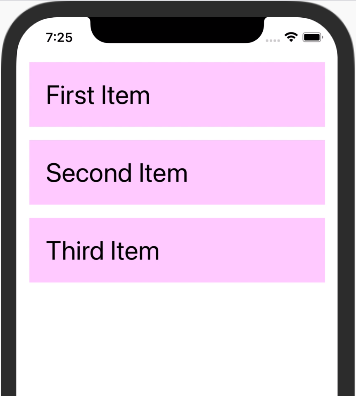
\includegraphics[width=0.49\textwidth]{figures/safeareaview.png}}
\subfigure[Darstellung einer \textit{FlatList} ohne \textit{SafeViewArea}]{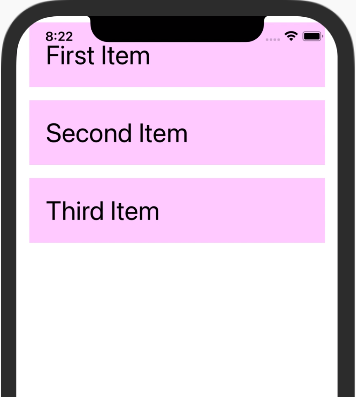
\includegraphics[width=0.49\textwidth]{figures/no_safeareaview.png}}
\caption{Exemplarische Darstellung einer Liste mit \textit{FlatList} in iOS}
\label{fig:flatlist:ios}
\end{figure}

Damit auf gewisse Funktionalitäten des Geräts zuzugreifen werden kann, benötigten Anwendungen teilweise die Erlaubnis des Nutzers.
Android unterscheidet dabei zwischen \glqq normal\grqq{} und \glqq dangerous\grqq{} \textit{Permissions}.
Beispiele für letzteres sind die \textit{android.permission.ACCESS\_""FINE\_LOCATION} oder \textit{android.permission.READ\_CONTA""CTS}.
Alle anderen \textit{Permissions} werden aus dem AndroidManifest.xml generiert.\\
Bei iOS Apps werden die benötigten Berechtigungen der App in XCode\footnote{Die \ac{ide} zur Entwicklung von iOS Anwendungen.} festgelegt und beim Installationsprozess abgefragt.
Nur wenn der Nutzer diese Berechtigungen akzeptiert, kann die Anwendung installiert werden.
Daher wird in der App für die Nutzung von Funktionalitäten wie Standort- oder Kontaktzugriff keine zusätzliche Erlaubnis des Nutzers benötigt.

\section{Installation}
Das Ziel dieser Funktionalität ist es, dass die Anwendung auf das mobile Endgerät des Nutzers installiert werden kann.

\subparagraph{Progressive Web App\\}
Um eine Webanwendung installierbar zu machen, benötigt sie ein App Manifest und \textit{HTTPS}.
Für chromiumbasierte Browser ist außerdem ein Service Worker notwendig.
Dort bedeutet das Installieren in neueren Browserversionen, dass eine sogenannte WebAPK aus dem App Manifest generiert wird.
Somit ist diese dann auch unter allen Apps im App Drawer und den Einstellungen aufgelistet.
Dennoch ist sie Teil von Chrome und verliert beispielsweise ihre Daten, wenn die Cache-Daten von Chrome geleert werden.
Bei iOS Geräten bedeutet das Installieren lediglich ein Lesezeichen für die Anwendung zum Startbildschirm des mobilen Endgeräts hinzuzufügen, wie es auch mit herkömmlichen Webseiten und -anwendungen möglich ist.
Deshalb erscheint die App weder im App Drawer, noch unter den Einstellungen.

Wie bereits im Kapitel \ref{ch:basics} angemerkt, handelt es sich bei dem App Manifest um eine \ac{json}-Datei, die Informationen über die Anwendung bereitstellt.
Um das Installieren zu ermöglichen, muss dieses die in Abbildung \ref{lst:manifest} gezeigten Attribute beinhalten.
Ersteres gibt an, wie die Anwendung dargestellt werden soll.
Damit sie einer mobilen App gleicht, wird hier der Wert \textit{standalone} oder \textit{fullscreen} empfohlen.
Dadurch verschwindet die für Webanwendungen übliche \ac{url}-Leiste.
Durch die Angabe einer \textit{background\_color} erhält die Anwendung eine Hintergrundfarbe beim Starten der App.
Diese wird angezeigt, bis Stylingsheets oder Hintergrundbilder der PWA geladen sind.
Das \textit{icons}-Attribut besitzt ein Array aus Objekten, welche die Dateipfade der Icons in verschiedenen Größen angeben.
Die \textit{start\_url} gibt die relativen \ac{url} an, die beim Starten der installierten Anwendung geöffnet werden soll \cite{MDNcontributors.d}.\\
Das Manifest wird per \glqq <link>\grqq{}-Tag in die index.html eingebunden und dessen Informationen sind danach auch im Application-Tab der Google Developer Tools einsehbar \cite{Caceres.2021}.

\begin{lstlisting}[language=Java,caption={Fertiges App Manifest der PWA},captionpos=b,label={lst:manifest}]
{
  "name": "COVID-19 Fallzahlen",
  "icons": [
    {
      "src": "favicon.ico",
      "type": "image/x-icon",
      "sizes": "64x64",
    },
    {
      "src": "logo192.png",
      "type": "image/png",
      "sizes": "192x192"
    },
    {
      "src": "logo512.png",
      "type": "image/png",
      "sizes": "512x512"
    }
  ],
  "start_url": ".",
  "display": "standalone",
  "background_color": "#ffffff"
}
\end{lstlisting}

Wichtig ist dabei, dass das Manifest als experimentell markiert ist, da es nicht von allen mobilen Browsern und Betriebssystemen komplett unterstützt wird.
Aktuell betrifft das Safari, welches das Installieren aus Browsern, die auf iOS statt mit ihrem eigenen HTML-Renderer mit WebKit\footnote{HTML-Renderer von Safari.} laufen (Chrome, Firefox und Opera), nicht unterstützt \cite{Deveria.o.J.}.
Denn jede iOS App muss laut Punkt 2.5.6 der Apple App Store Review Guidelines als Engine WebKit nutzen \cite{Apple.07.06.2021}.

Wenn der Nutzer nun die Anwendung im Browser aufruft, kann er sie auf browserabhängige Weise installieren und somit mit einem Klick vom Startbildschirm oder App-Drawer aus öffnen.
Beim Aufrufen der Seite, öffnet sich im Chrome Browser auf Android außerdem eine Installationsaufforderung für die App am unteren Bildschirmrand.
Diese zusätzliche Funktionalität muss aktuell für den Safari Browser explizit implementiert werden.

Für das Ermöglichen von Aktualisierungen der \ac{pwa} muss keine weitere Programmierung vorgenommen werden.
Sobald ein neues Deployment\footnote{Veröffentlichung der Webseite.} der Anwendung vorgenommen wird, ist sie automatisch auf dem neusten Stand, selbst wenn die \ac{pwa} installiert ist.

\subparagraph{React Native App\\}
Zur Ermöglichung der Installation einer React Native App bedarf es keiner konkreten Implementierung.
Es muss nur  -- wie bei nativen Anwendungen -- die betriebssystemabhängige Signierung durchgeführt werden.
Durch diesen Prozess erhält die Anwendung einen \textit{Release key} und einen \textit{Upload Key}, durch die sie eindeutig identifizierbar ist und auf die alle zukünftigen Aktualisierungen referenziert werden.
Die genauen Schritte sind in den offiziellen Dokumentationen von Apple und Android nachzulesen.
Zusätzliche Schritte für iOS, die eine Besonderheit von React Native sind, sind das Verbieten von HTTP Anfragen und das Umstellen der App im \textit{Release}-Schema.
Danach kann die resultierende \ac{apk}-Datei in den Google Play Store oder die \ac{ipa}-Datei in den Apple App Store hochgeladen werden.
Dort werden sie getestet und verifiziert.
Zuletzt kann der Nutzer sie im jeweiligen Store suchen und herunterladen.

Ähnlich wie bei der \ac{pwa} gibt es bei Android Apps die \textit{AndroidManifest.xml}-Datei, welche Informationen zur Installation der App bereitstellt, wie das App Icon, Berechtigungen der App oder die mindestens benötigte Android Version.
Bereits bei der Installation durch den Play Store wird dabei nach Berechtigungen für die Nutzung der App gefragt, die aus der AndroidManifest.xml ausgelesen werden.
Bei iOS Apps ist das die \textit{Info.plist}-Datei.

\section{Offlinebetrieb}
Die Anwendung soll auch ohne Internetverbindung aufrufbar, mit Daten gefüllt und die Funktion des Durchsuchens nutzbar sein.

\subparagraph{Progressive Web App\\}
Generell benötigten Nutzer eine Internetverbindung, um auf Webanwendungen zuzugreifen.
Durch moderne Webschnittstellen ist mittlerweile auch den Offlinebetrieb ermöglichen.
Hierfür wird der Service Worker genutzt.
Er kann auf eine statische, individuelle Seite weiterleiten, welche die standardmäßig angezeigte Seite bei fehlender Internetverbindung ersetzt.
Alternativ können aber durch den Service Worker auch Daten abgespeichert und im Offlinebetrieb angezeigt werden.
Hierfür gibt es neben der bereits seit 2015 bestehenden \textit{IndexedDB} auch die Cache \ac{api}, mit der Daten als Request-Response-Paar abgespeichert werden können.
Aus einer Vielzahl von clientseitigen Speichermechanismen im Web (\textit{LocalStorage}, \textit{SessionStorage} oder \textit{Cookies}) eignen sich speziell diese beiden zur Nutzung in einer \ac{pwa}.
Das ist damit zu begründen, dass sie persistent sein können und asynchron ablaufen \cite{LePage.2020}.
Letzteres verhindert, dass der Main Thread der Webanwendung blockiert wird und die Nutzer unter Umständen lange Warte- /Ladezeiten bei der Bedienung der Anwendung erfahren.
Gerade die Cache \ac{api} wird jedoch im Zusammenhang mit \acp{pwa} besonders empfohlen, weil diese im Gegensatz zur \textit{IndexedDB} auch statische Ressourcen speichert \cite{MDNcontributors.o.J.}.
Die Speichergröße von beiden Speichern ist abhängig von dem Browser, in dem die Webanwendung aufgerufen wird.

Durch das Zwischenspeichern der Daten wird ermöglicht, dass die \ac{pwa} dem Nutzer selbst ohne oder mit schlechter Internetverbindung Rückmeldung in Form einer Benutzeroberfläche zur Verfügung stellt.
Das kann entweder eine individuelle Seite oder dieselbe Seite mit veralteten Daten sein.
Ferner ist das Caching der Daten zum Offlinebetrieb der Anwendung nicht nur hilfreich, wenn keine Internetverbindung besteht, sondern reduziert auch allgemein die Anfragen an den Server. %Quelle

Eine Anwendung kann mehrere Caches besitzen, die zur Unterscheidung benannt werden.
In der programmierten \ac{pwa} werden an zwei Stellen Daten im \textit{cache-v1}-Cache gespeichert.
Zuerst geschieht dies beim Installieren des Service Workers im \textit{install}-Lifecycle-Event.
Hier werden statische Ressourcen wie das Manifest und Bilddateien in den Cache aufgenommen.\\
Die zweite Stelle ist während des \textit{fetch}-Events zur Speicherung von Netzwerkabfragen.
Dabei ist nicht nur die Speicherung von Bedeutung, sondern auch wie dieses Cache-Daten in der \ac{pwa} genutzt werden.
Hierfür definiert Jake Archibald mehrere Strategien, wovon die \glqq Cache, falling back to network\grqq{}-, \glqq Network, falling back to cache\grqq{}- und \glqq Cache then network\grqq{}-Strategie ausgewählt und für diesen Anwendungsfall untersucht wurden \cite{Archibald.2020}.

\begin{figure}
\centering
    \subfigure[Cache, falling back to network]{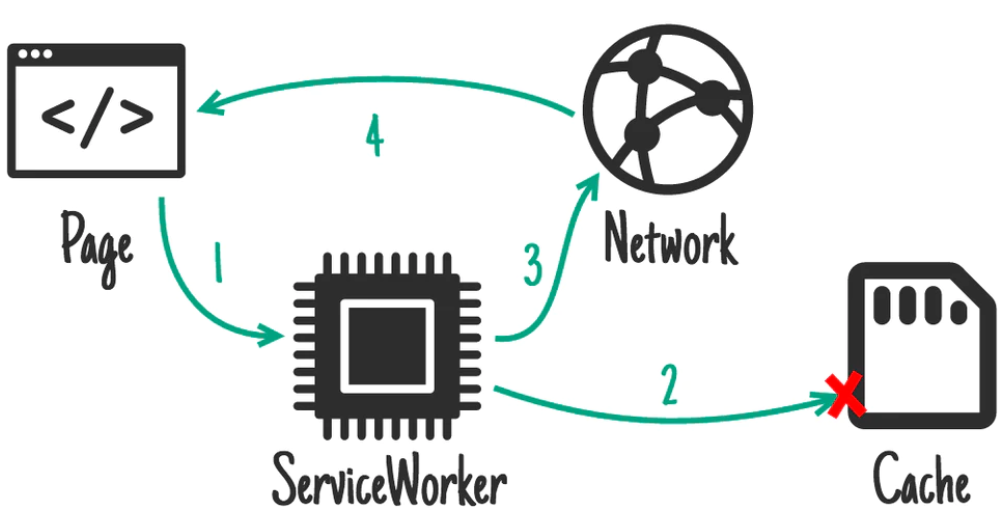
\includegraphics[width=0.49\textwidth]{figures/Cache_falling_back_to_network.png}}
        \subfigure[Network, falling back to cache]{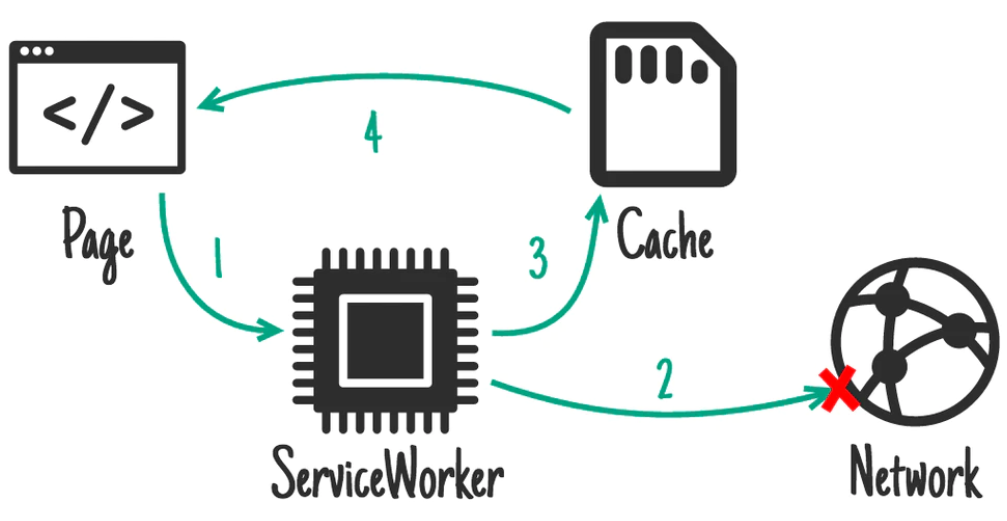
\includegraphics[width=0.49\textwidth]{figures/Network_falling_back_to_cache.png}}
    \subfigure[Cache then network]{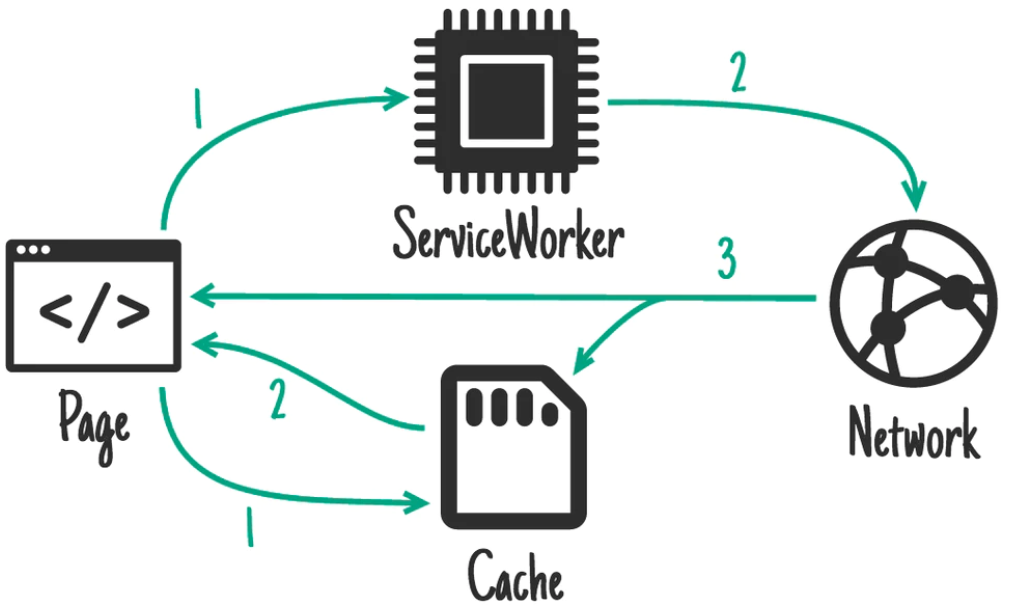
\includegraphics[width=0.49\textwidth]{figures/Cache_then_network.png}}
\quelle{\cite{Archibald.2020}}
\caption{Speichermanagementstrategien}
\end{figure}

Ersteres bedeutet, dass der Service Worker beim Ausführen der Anwendungen zuerst prüft, ob die Daten im Cache-Speicher verfügbar sind, und wenn dies nicht zutrifft, eine Netzwerkanfrage stellt.
Die Anwendung ist dadurch performant, der Nachteil ist jedoch, dass die Daten beim Aufrufen der App nicht auf dem aktuellsten Stand sind.\\
Zweiteres verfolgt einen gegenteiligen Ansatz, bei dem nur im Falle einer fehlenden Netzwerkverbindung die Daten aus dem Cache verwendet werden.
Auf diese Weise sind die Daten stets aktuell, jedoch erhöht sich auch die Anzahl an Netzwerkanfragen und somit der Verbrauch von Datenvolumen, gerade bei dieser großen Datenmenge, die vom Robert Koch-Institut zur Verfügung gestellt wird.
Außerdem muss der Nutzer warten, bis die Netzwerkanfrage fehlschlägt, bis die Cache-Daten genutzt werden.
Dies kann für Nutzer mit geringer Internetverbindung länger dauern und dadurch die Nutzererfahrung verschlechtern.\\
Der \glqq Cache then network\grqq{}-Ansatz stellt gleichzeitig eine Anfrage an den Cache und eine an das Netzwerk.
Sobald die Daten aus dem Cache geladen sind, werden sie in der Anwendung dargestellt.
In jedem Fall werden die Daten aber auch nach Antwort der Netzwerkanfrage im Cache aktualisiert \cite{Archibald.2020}.
Diese Variante benötigt eine Implementierung im Service Worker und in der Anwendung selbst, um zwei Anfragen auszulösen.

Die Entscheidung fiel zuletzt auf den \glqq Cache then network\grqq{}-Ansatz, mit einer zusätzlichen Besonderheit.
Denn dadurch, dass bei der Anwendung einerseits die Aktualität der Daten eine große Rolle spielt, anderseits die Daten sich nicht über den Tag hinweg ändern, ist eine ständige zweite Anfrage an das Netzwerk redundant.
Deshalb ist in der Anwendung eine Abfrage implementiert, welche prüft, ob das Datum der Robert Koch-Institut-Daten mit dem heutigen übereinstimmt.
Nur wenn dies nicht zutrifft, wird eine Anfrage an das Netzwerk gestellt und daraufhin die Daten im Cache aktualisiert.

Durch das Zwischenspeichern der Daten wird ermöglicht, dass die \ac{pwa} dem Nutzer selbst ohne oder mit schlechter Internetverbindung Rückmeldung in Form einer Benutzeroberfläche zur Verfügung stellt.
Das kann entweder eine individuelle Seite oder dieselbe Seite mit veralteten Daten sein.
In der implementierten \ac{pwa} ist letzteres der Fall und über eine Zeitstempel erfährt der Nutzer die Aktualität der angezeigten Daten.
Hierbei ist wichtig anzumerken, dass der Offlinebetrieb nur dann gewährleistet ist, wenn der Service Worker bereits auf dem Gerät installiert ist.
Dies ist der Fall, wenn die Anwendung in einem Browser-Tab geöffnet ist oder auf den Startbildschirm heruntergeladen wurde.

\subparagraph{React Native App\\}
Mobile Anwendungen sind im Gegensatz zu \acp{pwa} generell offline aufrufbar.
Der Grund dafür ist, dass das Rendern der App nicht abhängig von einer Netzwerkverbindung ist, weil sie bereits auf dem Endgerät existiert.
Dennoch ist es sinnvoll, auch hier eine lokale Speicherung der Corona-Daten vorzunehmen, um diese trotz Offlinebetriebs anzeigen zu können.

Seit React Native Version 0.59 sind einige Komponenten als veraltet deklariert.
Das betrifft unter anderem \textit{AsyncStorage}\footnote{\url{https://github.com/react-native-async-storage/async-storage}} und \textit{NetInfo}\footnote{\url{https://github.com/react-native-netinfo/react-native-netinfo}}.
Sie wurden jedoch nicht entfernt, sondern lediglich aus der Kernbibliothek react-native exkludiert und in jeweils eigene Bibliotheken mit eigenen Verantwortlichen verschoben \cite{Turner.2019}.
Diese Bibliotheken sind dem GitHub Repository @react-native-community zu finden und benötigen nach der Installation per npm auch das React Native-spezifische \textit{Linkings}\footnote{Ein Prozess, bei dem diejenigen nativen Fähigkeiten, die von einer Bibliothek benötigt werden, der Anwendung hinzugefügt werden. Durch diesen zusätzlichen Schritt verringert sich die Größe der Basis Anwendungen, die eventuell keine nativen Funktionalitäten benötigt.}.

Der \textit{AsyncStorage} legt persistent Daten unverschlüsselt in einem lokalen Speicher ab.
Der Speicherplatz ist dabei standardmäßig auf 6 MB beschränkt, allerdings kann dieser auch manuell erweitert werden \cite{Behrends.2018}.
Die Daten werden bei iOS Geräten im \textit{Application Support}-Verzeichnis abgelegt.
In Android wird für die asynchrone Speicherung \textit{SQLite} verwendet.

Die Implementierung der Speicherung erfolgt nach der \glqq Network, falling back to cache\grqq{}-Strategie.
Demnach wird erst abgefragt, ob das Gerät eine aktive Internetverbindung besitzt und wenn dies fehlschlägt, die Daten aus dem \textit{AsyncStorage} verwendet.\\
Dafür stellt die \textit{NetInfo}-Komponente Informationen zur aktuellen Netzwerkverbindung bereit.
Diese wird genutzt um im Falle einer fehlenden Internetverbindung, die Corona-Daten aus dem \textit{AsyncStorage} zu entnehmen.\\
Zuerst werden jedoch die Daten nach erfolgreicher \ac{api}-Abfrage im \textit{AsyncStorage} gespeichert.
Eine Anforderung dabei ist, dass sie vorher in ein \ac{json}-String konvertiert werden müssen.

Im initialen \textit{useEffect}-Hook wird beim nächsten Aufruf der App geprüft, ob eine Internetverbindung besteht.
Wenn dies nicht zutrifft, wird per asynchroner Funktion auf die Daten im \textit{AsyncStorage} zugegriffen.
Sobald die Internetverbindung wiederhergestellt ist, werden die Daten per Netzwerkanfrage von der \ac{api} abgerufen.
%Außerdem wird ein weiterer \textit{useEffect} hinzugefügt, der auf Änderungen der \textit{NetInfo} hört und dementsprechend die Daten neu lädt.
%Somit wird gewährleistet, dass der Nutzer die neusten verfügbaren Corona-Daten erhält, wenn er eine Netzwerkverbindung hat.

Zum Testen des Offlinebetriebs muss nun das Internet des Rechners, auf dem der Emulator geöffnet ist, ausgeschaltet werden.
Dadurch wird nachgewiesen, dass die Anwendung trotz fehlender Netzwerkverbindung, die im \textit{AsyncStorage}-gespeicherten Corona-Daten anzeigen kann.

\section{Standortzugriff}
Anhand des Standorts soll der Nutzer die Liste der Landkreise nach dem Landkreis filtern, in dem er sich aktuell befindet.

\subparagraph{Progressive Web App\\}
Der Standortzugriff wird im Web über die sogenannte Geolocation \ac{api} ermöglicht.
Die Bestimmung erfolgt dabei unter anderem durch GPS und verschiedenste Netzwerksignale.
Sie wird vom \textit{navigator}-Objekt zur Verfügung gestellt und bietet unter anderem Zugriff auf Längen- und Breitengrad, Genauigkeit des bestimmten Standorts und die Höhe über dem Meeresspiegel des Gerätes \cite{Caceres.2021b}.

Zur Implementierung dieser Funktionalität wird der Nutzer beim Klicken des \glqq Standort bestimmen\grqq{}- Buttons zuerst, wie in Abbildung \ref{fig:permission_safari} zu sehen, nach seiner Zustimmung gefragt.

\begin{figure}[h]
 \centering
 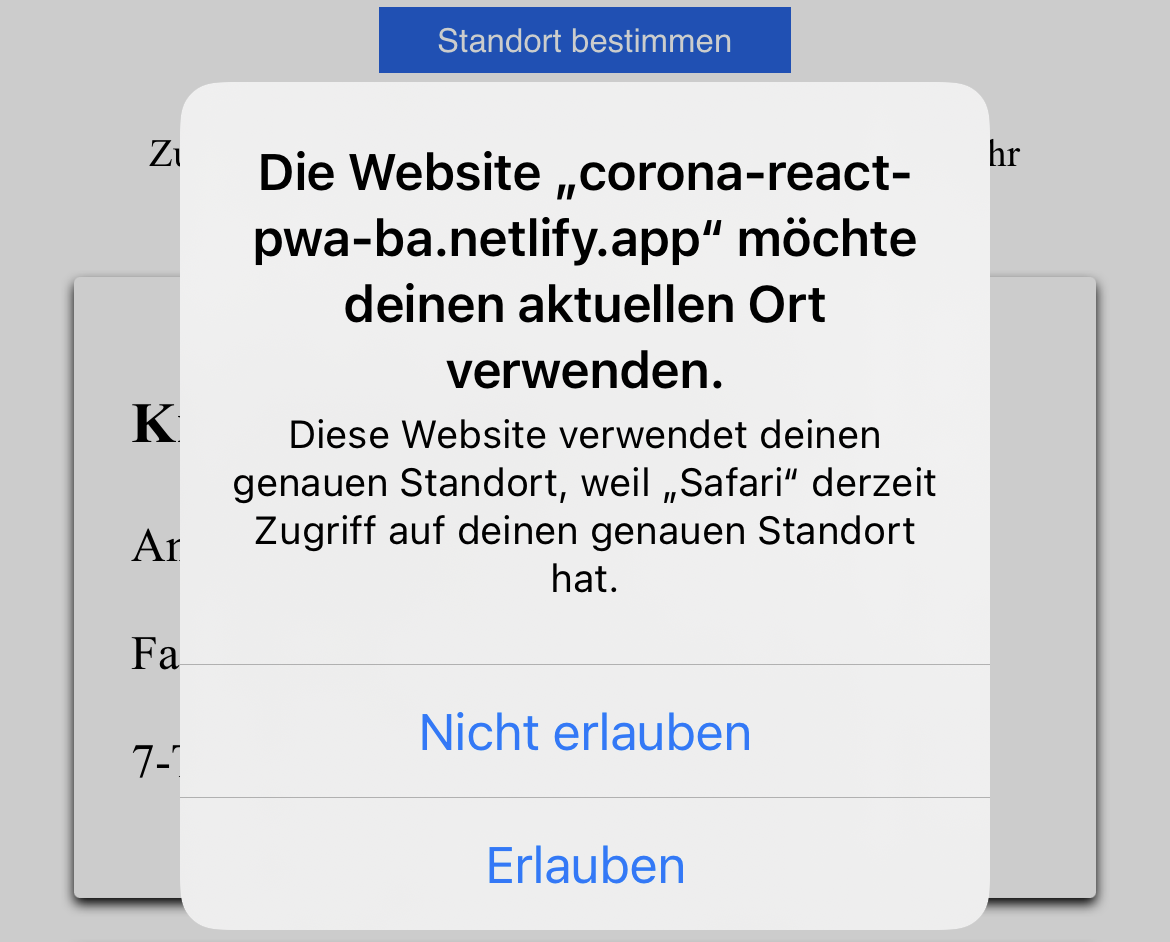
\includegraphics[width=0.6\textwidth]{figures/Permission_Safari.png}
 \caption{Erfragung des Standortzugriffs im iOS Browser}
 \label{fig:permission_safari}
\end{figure}

Sobald diese erteilt ist, wird die Methode \textit{Navigator.getCurrentPosition()} aufgerufen und deren Rückgabewert -- ein Objekt des Typs \textit{GeolocationPosition} -- einer Variablen zugewiesen.\\
Über eine kostenfreie Drittanbieter \ac{api} wird durch den Prozess des Reverse Geocodings aus den \textit{location.coords.latitude} und \textit{location.coords.longitude} Daten die Aufenthaltsstadt bestimmt.
Der Wert des \textit{input}-Feldes wird dann auf den ermittelten Landkreis gesetzt und die Liste der Landkreise automatisch nach dieser gefiltert.

\subparagraph{React Native App\\}
Zur Implementierung des Standortzugriffs in React Native wird die Community Lösung \textit{react-native-geolocation-service}\footnote{\url{https://github.com/Agontuk/react-native-geolocation-service}} verwendet, welche nach Aussage des Erstellers für Android und iOS programmiert ist.
Diese greift über eine \textit{Bridge} auf diejenigen Schnittstellen zu, die in Android und in iOS verantwortlich für den Standort sind.
In Android wird speziell wegen eines Timeout-Problems nicht auf die übliche \textit{Geocoder}-Klasse zugegriffen, sondern auf die \textit{FusedLocationProviderClient} \ac{api} des Google Play Services.
In iOS spricht die \textit{Bridge} den \textit{CLLocationMangager} des \textit{CoreLocation}-Modules an \cite{Agontuk.26.06.2021}.

Nach dem Installieren der Bibliothek muss für Android das Codefragment \textit{<uses-permi""ssion android:name=\"android.permission.ACCESS\_FINE\_LOCATION\"/>} in der AndroidManifest.xml hinzugefügt werden.
Das erlaubt der Anwendung auf den Standort zuzugreifen, wenn die App benutzt wird.
Da es sich beim Standortzugriff um eine \glqq dangerous\grqq{} \textit{Permission} handelt, muss zuerst der Nutzer dennoch erst eine Erlaubnis erteilen. 
Dies geschieht mit dem Befehl \textit{PermissionAndroid.request()}.
Für iOS wird neben dem Aktivieren des Standortzugriffs in XCode keine explizite Erlaubnis benötigt.

Die Abfrage der Erlaubnis erfolgt in der \textit{Search.js} in einem \textit{Effect}, welcher beim Öffnen der Anwendung ausgelöst wird.
Nach Zustimmung des Anwenders wird per \ac{api}-Anfrage an denselben Drittanbieter wie bei der \ac{pwa} der Name der Stadt aus den Daten über den Längen- und Breitengrad des Standorts des aktuellen Geräts erschlossen.\\
Hierbei ist zu betonen, dass im Normalfall bei nativen Anwendungen nach der Standortbestimmung auf die betriebssystemintegrierte Reverse Geocoding Funktion (beispielsweise bei Android die Geocoder \ac{api}) zurückgegriffen werden könnte.
In dieser Arbeit wird jedoch wegen der dadurch anfallenden Kosten darauf verzichtet.

Der logische Aufbau dieser Funktionalität konnte hier von der React \ac{pwa} übernommen werden, lediglich die Events wurden abgeändert.
So nennt sich das \textit{onChange}-Event einer Texteingabe in React nun \textit{onChangeText}-Event in React Native, während das \textit{input}-HTML-Element zum \textit{TextInput}-Tag wird.

\section{Kontaktzugriff}
Dem Nutzer soll es möglich sein, die Liste der Landkreise nach der Adresse eines Kontakts zu filtern.

\subparagraph{Progressive Web App\\}
Die Kontakte eines mobilen Endgeräts stehen der Webanwendung über das \textit{navigator}-Interface zur Verfügung.
Konkret ist es dessen \textit{contacts}-Property, dass in chromiumbasierten Browsern seit Version 80 die Contact Picker \ac{api} implementiert und im \ac{https} Kontext nutzbar ist.
Falls kein \ac{https} vorhanden ist, existiert das Property nicht im \textit{navigator}.

Mittels der \textit{select}-Funktion kann ein Kontakt auf Basis des Namens ausgewählt werden.
Dabei wird bei der Implementierung festgelegt, welche Kontaktdaten bei der Auswahl angezeigt werden.
In der \ac{pwa} soll nun aus der Adresse des Kontakts die Stadt entnommen und dieser Wert in das Suchfeld gesetzt werden.
Dadurch wird die Liste der Landkreise nach der Stadt der Adresse des Kontakts gefiltert.
Die \textit{address} eines Kontakts besitzt die gleichen Werte wie die des \textit{PaymentAddress}-Interfaces, das aus der Payment Request \ac{api} bekannt ist.
Diese sind beispielsweise \textit{city}, \textit{country} und \textit{region}.

Auch für diesen Eingriff in die Kontaktliste des Nutzers muss explizit eine Erlaubnis erteilt werden.
Die Abfrage erfolgt beim Betätigen des Buttons und ist wie beim Standortzugriff eine browserbasierte Abfrage.

Das Implementieren dieser Funktionalität gestaltet sich als problematisch, da die Contact Picker \ac{api} lediglich auf mobilen Browsern zur Verfügung steht.
Deshalb wurde die Funktion vollständig mit dem Android Emulator programmiert.
Dafür wird statt durch \url{http://localhost:3000} mit der IP-Adresse auf die laufende Webanwendung zugegriffen.
Doch auch hier gibt es Komplikationen mit der Unterstützung des \textit{contacts}-Attribut im \textit{navigator}.
Zuletzt hat lediglich das Deployment der \ac{pwa} geholfen, auf die Kontakte zuzugreifen.
Grund dafür kann sein, dass die Contact Picker \ac{api} nur mit \ac{https} verfügbar ist, jedoch sollte das nicht für \textit{localhost} gelten, wie bei der Implementierung der bisherigen Funktionalitäten.
Durch die Bestätigung der Sucheingabe wird in einer Funktion der Code in Abbildung \ref{lst:contacts} ausgeführt.

\begin{lstlisting}[language=Java,caption={Zugriff auf Kontakte},captionpos=b,label={lst:contacts}]
const props = ["name", "address"];
if ("contacts" in navigator) {
	try {
		const contact = await navigator.contacts.select(props, {});
        onQueryChange(contact[0].address[0].addressLine[0]);
		// Further processing
	} catch (ex) {
		// Handle any errors here.
	}
} else {
	// Handle no support
}
\end{lstlisting}

Mit dem Befehl \textit{navigator.contacts.select(props,{})} kann auf die Kontaktliste eines Geräts zugegriffen werden.
Der erste Übergabeparameter ist dabei ein \textit{Array} mit denjenigen Attributen, welche angezeigt werden sollen, während der Zweite weitere Konfigurationen wie beispielsweise eine Mehrfachauswahl von Kontakten zulässt.
Der Rückgabewert ist in diesem Falle ein \textit{Array}, dass einen Kontakt enthält.
Per \textit{address[0]} wird auf die erste Adresse des Kontakts zugegriffen.
Eigentlich kann daraufhin durch \textit{.city} die Stadt dieser Adresse erreicht werden, jedoch erlaubt der verwendete Emulator bei der Erstellung eines Kontakts nur die Eingabe der Adresse in eine Eingabezeile.
Deshalb wird hier auf die Adresszeile zugegriffen, in der zur Vereinfachung aktuell nur die Stadt notiert ist.
Dieser Wert wird nach Bestätigung der Auswahl direkt in das Suchfeld übernommen und die Liste der Landkreise somit nach dieser Stadt gefiltert.

\subparagraph{React Native App\\}
Bei der React Native App wurde dies mit der Bibliothek \textit{react-native-contacts}\footnote{\url{https://github.com/morenoh149/react-native-contacts}} umgesetzt.
Diese greift in Android auf die \textit{ContactsContract} Klasse und in iOS auf die \textit{CNContact} zu.

Nach der Installation der Bibliothek müssen in der AndroidManifest-Datei erneut eine \textit{uses-permissions} ergänzt werden, in diesem Fall die \textit{android.permission.READ\_""CONTACTS}-Erlaubnis für das Lesen der Kontakte.
Da es sich auch hierbei um ein \glqq dangerous\grqq{} Berechtigung handelt, muss erneut zuerst nach der Erlaubnis des Nutzers gefragt werden.
Dies wird in einer \textit{asnyc}-Funktion erledigt.
Sie wird in einem \textit{Modal} aufgerufen, in dem nach dem Namen des gesuchten Kontakts gefragt wird.
Nach der Betätigung des \textit{Bestätigen}-Buttons wird nun mit der Funktion \textit{Contact.getContactsMatchingString(text)}, die als Übergabeparameter einen \textit{string} annimmt, ein Kontakt gesucht, der diesen Übergabeparameter als Teil seines Namens enthält.\\
Das Ergebnis ist ein \textit{Array} aus Objekten von Kontakten, auf die das Kriterium zutrifft.
Zur Vereinfachung der Implementierung wird nur der erste Kontakt betrachtet und aus dessen \textit{postalAddresses} die erste Adresse ausgewählt.
Diese wird dann per Aufruf von \textit{onQueryChange} automatisch in das Suchfeld gesetzt und somit die Liste der Landkreise nach dieser Stadt gefiltert.\\
Bei der Implementierung wurde einige Mal keine Daten angezeigt und die Console beinhaltete \glqq {"\_U": 0, "\_V": 0, "\_W": null, "\_X": null}\grqq{}.
Es stellte sich heraus, dass dies damit verbunden ist, dass beim Anfordern der Ressourcen nicht auf das Auflösen des \textit{Promises} gewartet wurde.
Das konnte mit dem Schlüsselwörtern \textit{await} in den asynchronen Funktionen gelöst werden.

\section{Benachrichtigungen}
Die entwickelte App soll seinen Abonnenten Benachrichtigungen senden können.
In diesen können beispielsweise aktuelle Veränderungen der Inzidenz oder Informationen über neue Fallzahlen angezeigt werden.

Wie in Kapitel \ref{ch:basics} beschrieben, lassen sich Benachrichtigungen in nicht-persistente und persistente Benachrichtigungen unterteilen.
Im Zuge dieser Arbeit soll nun erklärt werden, wie letzteres umgesetzt werden kann, da diese eine höhere Relevanz zur Interaktion mit dem Nutzern bieten und hierfür auch Schnittstellen genutzt werden, die von nicht-persistente Benachrichtigungen verwendet werden.
Somit wird auf die Nutzung beider Arten eingegangen.

Für beide Anwendungen muss ferner das Management der Nutzererlaubnis implementiert werden.
Dies wird zur Begrenzung des Umfangs in der Arbeit exkludiert und im Folgenden lediglich auf die Programmierung der Push Benachrichtigungsfunktion selbst eingegangen.

\subparagraph{Progressive Web App\\}
\begin{figure}[h]
 \centering
 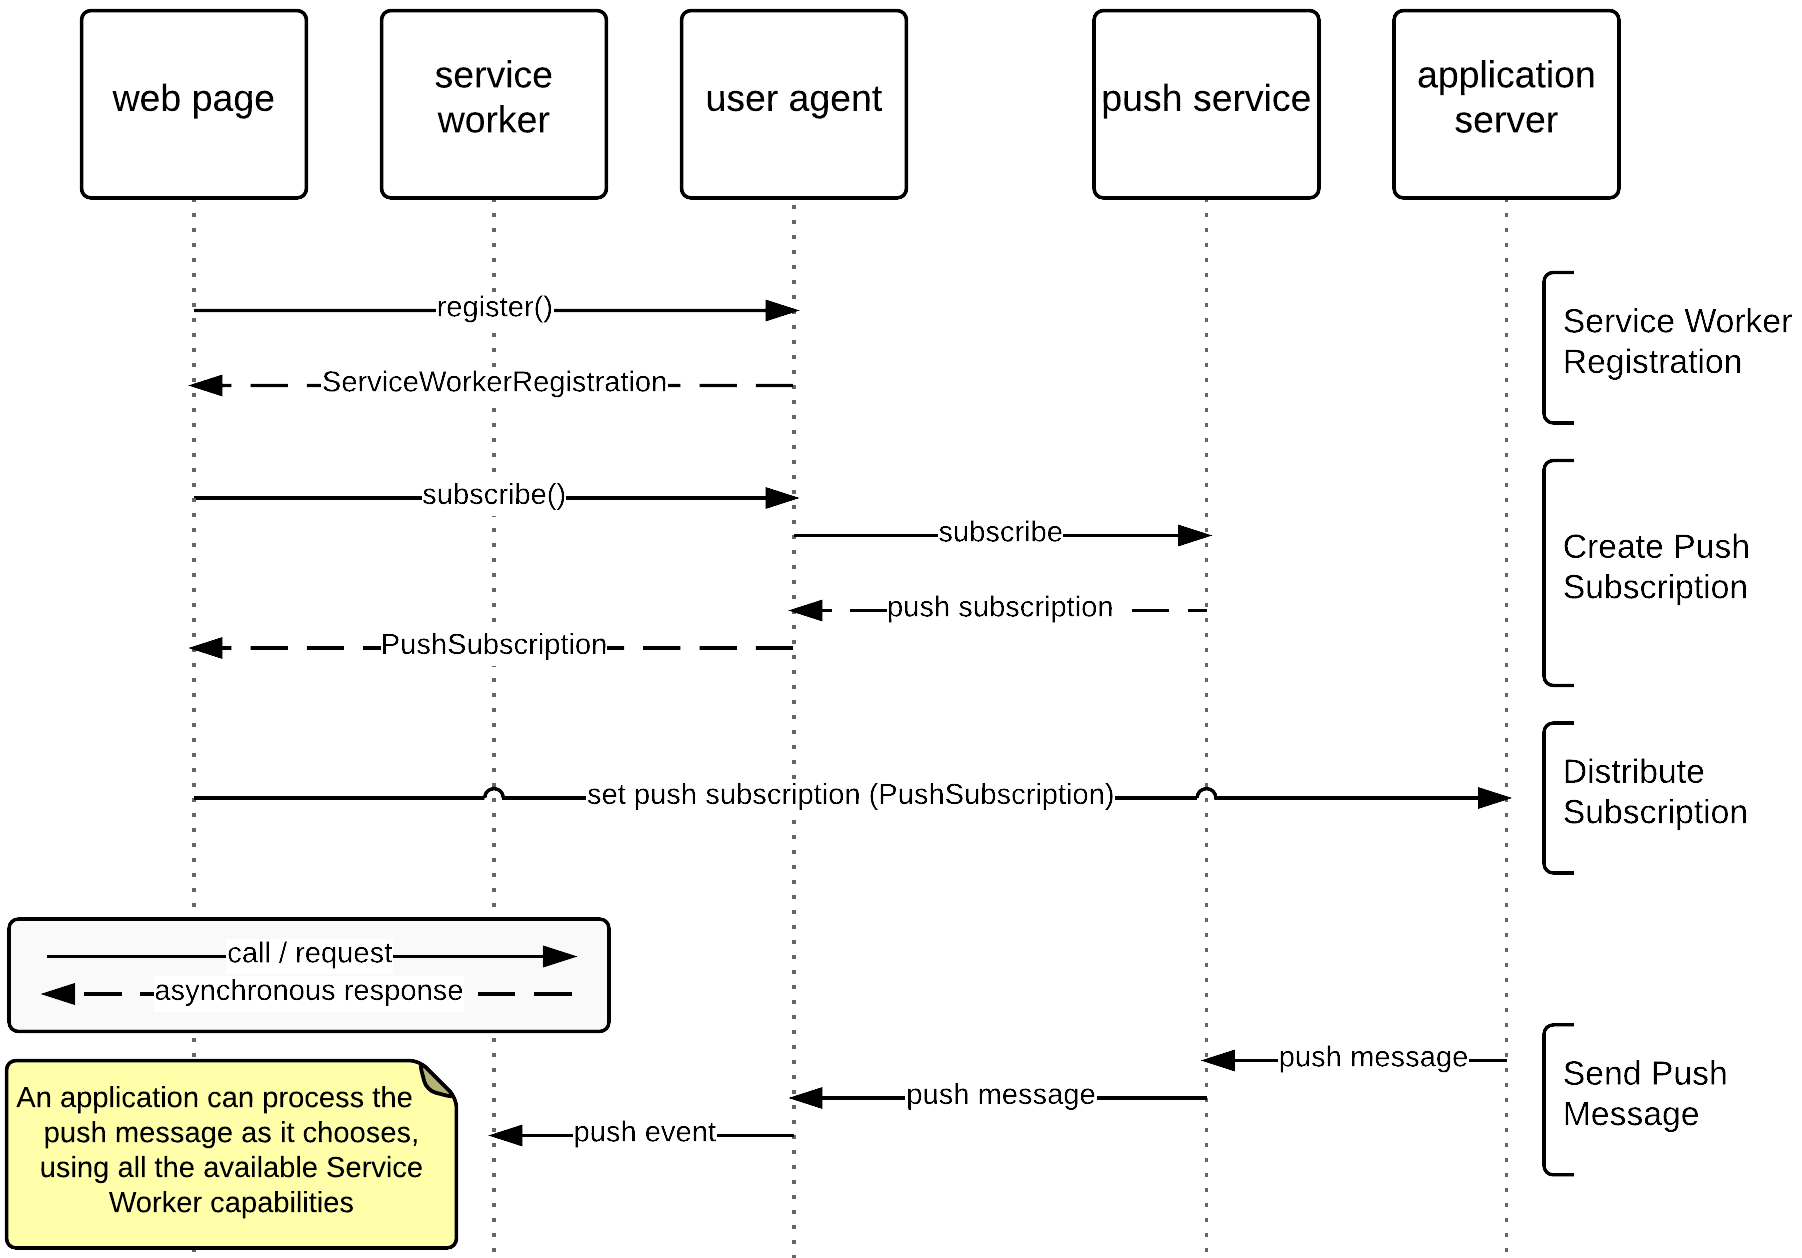
\includegraphics[width=1\textwidth]{figures/sequence_diagram_web_push.png}
 \quelle{\cite{MozillaWiki.2016}}
 \caption{Ausschnitt eines Sequenzdiagramms des Web Push Prinzips}
 \label{fig:structure_webpush}
\end{figure}

Zum besseren Verständnis der Implementierung soll zuerst das Web Push Prinzip umrissen werden.
Der Name Push bezieht sich darauf, dass keine Aktion vom Client vorgenommen werden muss, um diese Informationen vom Server zu erhalten.
Wie auf der rechten Seite in der Abbildung \ref{fig:structure_webpush} dargestellt, besitzt das Konzept vier Abschnitte.\\
Die erste Station betrifft die Installation des Service Workers.
Dieser wird benötigt, um Push Benachrichtigungen im Hintergrund zu erhalten, da er unabhängig von der Anwendung selbst aktiv ist und somit immer auf einen Push reagieren kann.\\
Die zweite Station findet im \textit{UserAgent}, also auf Clientseite statt.
Um Push Benachrichtungen zu ermöglichen, muss hier die Erlaubnis des Nutzers abgefragt werden.
Wird dies erlaubt, wird durch eine \textit{PushSubscription} ein Abonnement für das Gerät des aktuellen Nutzers erstellt.
Dieses Abonnement wird benötigt, um das Endgerät eindeutig zu identifizieren und somit für spätere Aktionen verfügbar zu machen.
Deshalb wird das \textit{PushSubscription}-Objekt an das Backend oder den Server versendet, um dort in einer Datenbank abgespeichert zu werden.
All dies ist Bestandteil der Push \ac{api}.\\
Die dritte Station umfasst das Auslösen einer Push Benachrichtigung in einem Backend.
Hier muss ein \ac{api}-Aufruf an einen Push Service getätigt werden, in dem alle nötigen Informationen zum Inhalt und Empfänger der Push Benachrichtigung vorhanden sind.
Dieser Aufruf wird bezeichnet als \textit{Web Push Protocol}, welches durch einen IETF\footnote{Internet Engineering Task Force. Eine Organisation, die Web-Standards entwickelt.}-Standard definiert ist.
Der Push Service ist Teil eines jeden Browsers zur Verwaltung von Push Benachrichtigungen und ist deshalb dessen Implementierung überlassen.
Jedoch ist festgelegt, dass der Service stets Anfragen in Form des \textit{Web Push Protocols} verarbeiten kann, wodurch für Entwickler die Form des Push Services irrelevant ist.\\
Die letzte Station behandelt das \textit{Push}-Event auf dem Endgerät, welches die empfangenen Daten verarbeitet und daraus eine Benachrichtigung erzeugt.
Dies wird von der Notification \ac{api} abgedeckt, welcher Zugriff auf die betriebssystemsspezifischen Benachrichtungsfunktionen besitzt.
Hierfür wird im Event die Anweisung \textit{self.registration.showNoti\-fication(title, options)} ausgeführt.
Der Übergabeparameter \textit{title} ist dabei der Titel der Benachrichtigung und \textit{options} ein Objekt mit einer Vielzahl von Optionen wie der Text der Benachrichtigung, Aktion-Buttons, Icons und Vibrationsanweisungen.%Quelle
Im Service Worker eine Webanwendung kann auf dieses Event reagiert werden und aus den Informationen, die vom Push Service gesendet werden, eine lokale Benachrichtigung erzeugen.
Dies ist auch möglich, wenn die \ac{pwa} geschlossen ist, da der Service Worker unabhängig von der Anwendung selbst aktiv ist.
Eine aktive Internetverbindung ist jedoch unabdingbar, da der Push Service die Benachrichtigung sonst so lange einbehält, bis wieder eine Verbindung besteht.

Um den Fokus für diese Arbeit darauf zu richten, wie das Erhalten von Benachrichtigungen bei \acp{pwa} implementiert wird, wird der Backend-as-a-Service \textit{Firebase} genutzt.
Wichtig ist dabei, dass diese Funktionalität auch komplett selbst implementiert werden könnte, indem ein eigener Webserver mit beispielsweise Node.js aufgesetzt wird.
\textit{Firebase} wird von Google zur effizienten Implementierung eines Backendsystems zur Verfügung gestellt.
Speziell werden dessen Dienste \ac{fcm} und die Real Time Database genutzt.
Über dessen Konsole können einmalige sowie regelmäßige Benachrichtigungen an alle registrieren Nutzer versendet werden.
Da im Rahmen dieser Arbeit kein komplettes Management von Benachrichtigungen behandelt werden soll, werden die \textit{Keys} des \textit{PushSubscription}-Objekts lediglich in der Real Time Database abgelegt.
Daraufhin können über die \textit{Firebase} Console manuell Push Benachrichtigungen an alle \textit{Keys} versendet werden.

Damit Benachrichtigungen in der Anwendung empfangen werden können, muss erst die Erlaubnis des Nutzers erfragt werden.
Dies geschieht durch die Notification \ac{api} über den Aufruf von \textit{Notification.requestPermission()} beim Klicken des \glqq Fallzahlen abonnieren\grqq{}-Buttons.
In der asynchronen Rückgabe Funktion wird durch die \textit{messaging.getToken()}-Funktion von \textit{Firebase} ein Token für das Gerät generiert.
Im Service Worker wird dann im Falle eines Pushes vom Server im \textit{push}-Event durch die \textit{showNotification(title, body)}-Funktion eine Benachrichtigung entsendet.
\textit{Firebase} ersetzt die Nutzung des \textit{push}-Events jedoch durch seine eigene \textit{messaging.setBackgroundMessageHandler()}-Funktion, in der dasselbe durchgeführt wird.

Eine Besonderheit von der Nutzung des \ac{fcm} ist außerdem, dass dem App Manifest das Attribut \textit{gcm\_sender\_id} mit dem Wert der Sender ID hinzugefügt werden muss.
Diesen steht unter den Einstellungen des \textit{Firebase}-Projekts.%???

\subparagraph{React Native App\\}
Der Prozess von Push Benachrichtigungen ist bei Native Apps ähnlich aufgebaut.
Der Push Service ist hier jedoch nicht browser- sondern betriebssystemabhängig und bezeichnet sich als \textit{Operating system push notification service (OSPNS)}.
Bei Android Geräten werden Push Benachrichtigung von dem Google Cloud Messaging (heute Firebase Cloud Messaging) verwaltet und für iOS gibt es den \ac{apn}.
Native Anwendungen benötigen wie \acp{pwa} eine Internetverbindung zum Empfangen von Push Benachrichtigungen.

Auch bei der React Native Applikation wird zur Vereinfachung des Prozesses das \ac{fcm} von \textit{Firebase} verwendet, zumal es \ac{apn} integriert.
Dafür wird die Bibliothek \textit{react-native-firebase}\footnote{\url{https://github.com/invertase/react-native-firebase}} genutzt, die Push Benachrichtigungen an Android und iOS ermöglicht.
In dieser Arbeit wird jedoch nur exemplarisch auf die Einrichtung von \ac{fcm} mit iOS eingegangen.
Die Native App greift nach erfolgreicher Einrichtung, die wie bei der \ac{pwa} abläuft, auf dieselbe Real Time Database zu wie die \ac{pwa}.

Push Benachrichtigungen sind eine der Funktionen, für die keine explizite Berechtigung auf Android Geräten vorhanden sein muss.
Auf der anderen Seite wird dies von der verwendeten Bibliothek nur für die iOS Implementierung benötigt.
Daher muss das Ergebnis der Funktion \textit{messaging().requestPermission()} abgefragt und dementsprechend Benachrichtigungen erlaubt oder verwehrt werden.

Auch bei nativen Anwendungen wird zwischen persistenten und nicht-persistenten Benachrichtigungen unterschieden.
Das unterscheidet sich bei der Implementierung insofern, dass das Auslösen einer Benachrichtigung nicht in der Komponente selbst mittels des \textit{messaging().onMessage()}-Funktionsaufrufs in einem \textit{useEffects} geschieht, sondern in der \textit{index.js}-Datei durch die \textit{messaging.setBackgroundMessageHandler()}-Funktion allgemein initialisiert wird.
Diese Implementierung ermöglicht nur das Empfangen von Push Benachrichtigungen, wenn die App im Hintergrund oder geschlossen ist.